The detection layer is the interface between the real-world and the system.  Its subsystems consists of sensors and these sensors take in data such as audio, and then is sent to the processing layer.  It is also controlled by the raspberry pi subsystem in the controller layer.

\subsection{Acoustic Array}
The acoustic array will consist of a hexagonal printed circuit board with six microphones located at each point of the hexagon. Internally the board will contain the audio to digital converter and be capable of processing the microphone inputs from the array and forwarding that information to a digital component for processing. These requirements are meant by a COTS device called ReSpeaker, which will be the component used to meet these requirements. The subsystem will detect audio inputs from the environment and forward the raw analog audio data to the ADC for processing.

\begin{figure}[h!]
	\centering
 	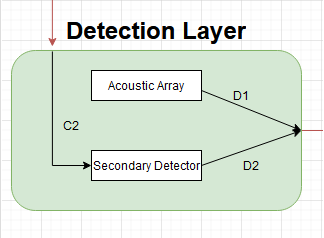
\includegraphics[width=0.50\textwidth]{images/detection}
 \caption{Acoustic Array}
\end{figure}

\subsubsection{Assumptions}
The ReSpeaker will detect across all six microphones and information will be compiled and properly forwarded to the ADC

\subsubsection{Responsibilities}
The subsystems sole purpose is to process raw audio data from the surrounding environment and compile it into a usable data stream. Each microphone works in tandem with the others to generate positional data, then forwards this information to the ADC to process and push further along the pipeline.

\subsubsection{Subsystem Interfaces}

\begin {table}[H]
\caption {Subsystem interfaces} 
\begin{center}
    \begin{tabular}{ | p{1cm} | p{6cm} | p{3cm} | p{3cm} |}
    \hline
    ID & Description & Inputs & Outputs \\ \hline
    \#RS01 & ReSpeaker Microphone Array & \pbox{3cm}{Microphone 1 \\ Microphone 2 \\ Microphone 3 \\ Microphone 4 \\ Microphone 5 \\  Microphone 6} & \pbox{3cm}{Compiled Audio Data to ADC}  \\ \hline
    \#RS02 & Power Supply & \pbox{3cm}{Power In} & \pbox{3cm}{N/A}  \\ \hline
    \end{tabular}
\end{center}
\end{table}

\subsection{Secondary Detector}
The secondary detector is instructed to activate by the raspberry pi when certain conditions are met; once it is activated, the data collected is sent to the ADC for analog to digital conversion.

\begin{figure}[h!]
	\centering
 	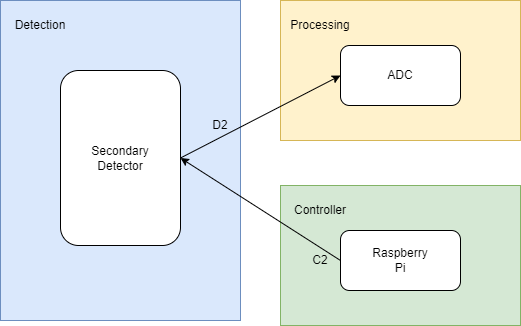
\includegraphics[width=0.60\textwidth]{images/secondary_detector_diagram.drawio}
 \caption{describes secondary detector's relation with the rest of the system}
\end{figure}

\subsubsection{Assumptions}
The secondary detector takes in some sort of sensory detail.  As of yet, this detail has not been determined 100\% yet; however, it will most likely be either some form of frequency detector or a visual detector.  If the secondary detector is to report to ODAS, then the sensory detail would be auditory.

\subsubsection{Responsibilities}
The main responsibility of the secondary detector is to be an extra method of detection, adding to the precision and accuracy.  It is on the standby of the raspberry pi and is processed the same way as the acoustic array.

\subsubsection{Subsystem Interfaces}
\begin {table}[H]
\caption {Subsystem interfaces} 
\begin{center}
    \begin{tabular}{ | p{1cm} | p{6cm} | p{4cm} | p{4cm} |}
    \hline
    ID & Description & Inputs & Outputs \\ \hline
    \#C2 & Activation of Secondary Detector & \pbox{3cm}{Raspberry pi signaling activation} & \pbox{3cm}{Secondary Detector activated}  \\ \hline
    \#D2 & Secondary Detector Data Sending & \pbox{3cm}{Analog data collected} & \pbox{3cm}{Data is sent to the ADC for digital conversion}  \\ \hline
    \end{tabular}
\end{center}
\end{table}